In diesem Kapitel wird ein bestehender Schnittstellentest analysiert. Der Schnittstellentest heißt bei \ac{zf} Quicktest.
Der Quicktest wird in Softcar ausgeführt, was ein Programm für \ac{sil} Tests ist, das von \ac{zf} entwickelt wurde.

Schnittstellen der Projekte in meiner Abteilung werden in einer \ac{xml} definiert, die Datafield heißt.
Wie in Abschnitt 2.1 beschrieben, werden \ac{xml} Daten an sich sowie der Zugriff auf jene im Sinne eines Schnittstellentests
überprüft. Der Quicktest bei \ac{zf} begrenzt sich auf den Test des Zugriffs. Um die Schnittstellen im C Code zu
verwenden, werden Makros aus der Datafield generiert. Mit den Makros kann auf die Signale zugegriffen werden (siehe Kapitel 4).
Die Verbindung zweier Signale, eine Schnittstelle, erfolgt durch den Einsatz der Makros. Der Quicktest überprüft, ob
diese Verbindung korrekt ist.

Das Flussdiagramm in Abbildung 3.1 gibt einen Überblick, was beim Aufruf des Quicktests ausgeführt wird.
Im Grunde genommen wird eine Quicktest.c, die die Schnittstellentests beinhaltet, generiert und mit dem Gesamtprojekt kompiliert. 
Die kompilierte \ac{exe} Datei wird in Softcar ausgeführt und fehlgeschlagene Tests
werden in eine Text-Datei als error log geschrieben \cite[vgl.][]{quicktestc}\cite[vgl.][]{quicktestlog}\cite[vgl.][]{datafield}.

  \begin{figure}[!h]
    \centering


  \begin{tikzpicture}%[every node/.style={rectangle,draw,text width=14em,align=center}]
    [
      % Stil für Ein- und Ausgabe
      io/.style={trapezium, trapezium left angle=70, trapezium right angle=110, fill=magenta!10, draw=magenta},
      % Stil für Operationen
      op/.style={rectangle, fill=orange!10, draw=orange},
      op4/.style={rectangle, fill=green!20, draw=green},
			op2/.style={rectangle, fill=green!20, draw=green, minimum height=2cm, minimum width=38mm},
			op3/.style={rectangle, fill=orange!10, draw=orange, minimum height=2cm, minimum width=38mm},
      % Stil für Entscheidungen
      cn/.style={diamond, aspect=2, inner sep=1pt, fill=red!10, draw=red, minimum width=20mm, minimum height=14mm},
      cn2/.style={diamond, aspect=2, inner sep=1pt, fill=blue!20, draw=blue, minimum width=20mm, minimum height=14mm},% Distanz zwischen den Knoten
      node distance=4mm]
    % Knoten
    \node[op4] (class) {Aufruf des Quicktests};
    
    \node[op4, below=of class] (init) {Generieren der Datafield};
    \node[op4, below=of init] (list) {Generieren der Quicktest.c};
    %\node[op, below=of list] (firstitem) {select first item in list};
%    \node[cn2, below=of list] (cond1) {};
    \node[op4, below=of list] (compile) {Kompilieren und Linken des Gesamtprojekts inklusive der Quicktest.c};
    \node[op4, below=of compile] (depnewlist) {Öffnen der Ergebnisse in Softcar};
%    \node[cn2, below=of depnewlist] (cond2) {};
    %\node[op, right=of cond2] (wrongdep) {select next item};
    %\node[op, below=of cond2] (makefiles) {search for item in dictionary to get makefiles};
    % \node[op4, below=of cond2] (initdep) {initialize object using item};
    % \node[op4, below=of initdep] (addobject) {add to object list};
    % \node[cn2, below=of addobject] (cond3) {\shortstack{last item from \\ dependency list?}};
    % \node[op4, right=of cond3] (wrongdep) {select next item};
    % \node[op4, below=of cond3] (findsubs) {object.findSubdirectories()};
    % \node[op4, below=of findsubs] (findfiles) {object.findFiles()};
    % \node[cn2, below=of findfiles] (cond4) {\shortstack{last item from\\ object list?}};
    % \node[op4, left=of cond4] (wrongobject) {select next item};
    % \node[op4, below=of cond4] (end) {Ende};
    
    \path[->]
		(class) edge (init)
		(init) edge (list)
		(list) edge (compile)
		(compile) edge (depnewlist);
      % (finddep) edge (depnewlist)
      % (depnewlist) edge (cond2)
      % (cond2) edge (initdep)
      % (initdep) edge (addobject)
      % (addobject) edge (cond3)
      % (cond3) edge node[above=0.2cm] {No}(wrongdep)
      % (cond3) edge node[right=0.2cm] {Yes} (findsubs)
      % (findsubs) edge (findfiles)
			% (findfiles) edge (cond4)
      % (cond4) edge node[above=0.2cm] {No}(wrongobject)
      % (cond4) edge node[left=0.5cm] {Yes} (end);

    % \draw[->] 
      % (wrongdep) --  ++(2,0) |- (cond2)
      % (wrongobject) -- ++(-2,0) |- (cond1);
		% \draw[->] (cond2) -- node[below] {Nein} ++(2.9,0) -- (entscheid);
		% \draw[->] (cond4) -- node[below] {Nein} ++(4.0,0) -| (gescheitert2);
		% \draw[->] (cond3) -- node[below] {Nein} ++(-4.0,0) -| (gescheitert3);
      %(wrongdep) edge (cond1);
			% (cond1) edge node[right] {Ja} (cond2)
			% (cond2) edge node[below] {Ja} (gesetz2);
    
    % \node[cn, align=center, below=of begehren] (cond1) {okay\\Unterschriften?};
		% \node[cn, align=center, below=of cond1] (cond2) {Landtag nimmt\\Gesetzentwurf an?};
		% \node[op3, align=center, right=of cond1] (gescheitert) {Volksbegehren\\gescheitert};
		% \node[op, align=center, right=of cond2] (entscheid) {Volksentscheid};
		% \node[io, below=of entscheid] (abstimmung) {Stimmen Sie ab!};
		% \node[cn, align=center, below=of abstimmung] (cond3) {Mehrheit stimmt\\mit Ja?};
		% \node[cn, align=center, below=of cond3] (cond4) {Mehr als ein Drittel\\aller Stimmberechtigten\\ stimmt mit Ja?};
		% \node[op2, align=center, below=of cond4] (gesetz) {Gesetz};
		% \node[op3, align=center, right=of gesetz] (gescheitert2) {Volksbegehren\\gescheitert};
		% \node[op3, align=center, left=of gesetz] (gescheitert3) {Volksbegehren\\gescheitert};
		% \node[op2, align=center, left=of cond2] (gesetz2) {Gesetz};
    % % Kanten
    % \path[->]
    %   (begehren) edge (cond1)
		% 	(entscheid) edge (abstimmung)
		% 	(abstimmung) edge (cond3)
    %   (cond3) edge node[right] {Ja} (cond4)
		% 	(cond4) edge node[right] {Ja} (gesetz)
		% 	(cond1) edge node[right] {Ja} (cond2)
		% 	(cond2) edge node[below] {Ja} (gesetz2);

    % \draw[->] (cond1) -- node[below] {Nein} ++(2.8,0) -- (gescheitert);
		% \draw[->] (cond2) -- node[below] {Nein} ++(2.9,0) -- (entscheid);
		% \draw[->] (cond4) -- node[below] {Nein} ++(4.0,0) -| (gescheitert2);
		% \draw[->] (cond3) -- node[below] {Nein} ++(-4.0,0) -| (gescheitert3);

  \end{tikzpicture}
  \caption{Quicktestaufruf \parencite[]{quicktestlog}}
  \end{figure}
  
  
  % \textbf{Bildinfo Quicktestdurchführung:
  % Überblick, was beim Quicktestaufruf passiert}
\newpage
\section*{Generieren der Datafield}
Datafield ist ein \ac{zf} interner Begriff. Jede Komponente besitzt eine Datafield, in der im Wesentlichen im \ac{xml} Format die Signale definiert werden.
Aus den Datafields der Komponente wird eine gesamte Datafield generiert, die die Signale aller Komponente beinhaltet \cite[vgl.][]{datafield}.

\section*{Generieren der Quicktest.c}
Schnittstellentests werden in diese Datei automatisiert geschrieben.
Folgende Daten werden dafür benötigt:
\begin{itemize}
\item Signale und deren Schnittstelleninformationen aus der Datafield \cite[vgl.][]{datafield}% (xml\_info.xml)
\item Funktionsaufrufe, in denen Schnittstellen definiert sind
\end{itemize}

Jede Schnittstelle wird mit Werten getestet, die in Abbildung 3.2 zu sehen sind.


\begin{figure}[h]
\centering
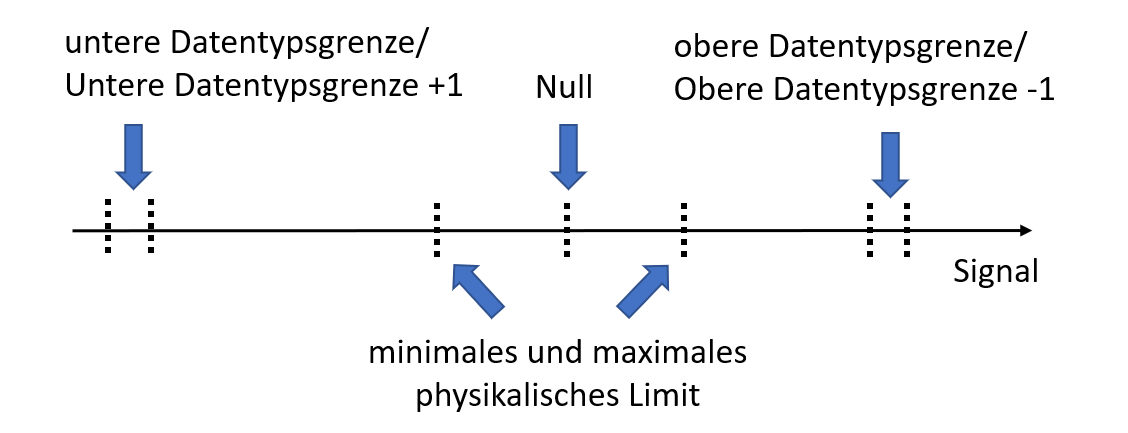
\includegraphics[scale=.9,]{Bilder/EquiZeitstrahl/QuicktestSignalstrahl.png}
\caption{Quicktest Werte auf einem Signalstrahl \cite[vgl.][]{quicktestc}}
\end{figure}
Es werden jeweils die untere und obere Datentypsgrenze als Werte genommen. Das ist im Sinne einer Grenzwertanalyse, denn
Grenzwerte verursachen oft ein fehlerhaftes Verhalten \cite[vgl.][S. 36]{integration}. 
Es wird jeweils eine Ganzzahl unter der oberen und eine Ganzzahl über der unteren Grenze getestet. Die Null wird auch getestet.
Ein physikalisches Limit kommt hier auch vor. Das ist ein Relikt, in dem eine Konvertierung und Skalierung zwischen zeitdiskreten Werten auf den vollen
Datentypsbereich stattfand. Es hat jetzt keine Bedeutung mehr.\par% und muss nicht mehr getestet werden.

In Abbildung 3.3 ist ein Flussdiagramm zu sehen. Es zeigt die Logik eines Schnittstellentests, wie sie in der Quicktest.c 
geschrieben ist. 
Im späteren Verlauf wird der Einfachheit halber ein Ein- und Ausgangssignal gesprochen, die im Folgenden kurz erklärt werden.
\begin{description}
\item[Ausgangssignal] Ein Signal, das aus der ersten Komponente austritt.
\item[Eingangssignal] Ein Signal, das in die zweite Komponente eintritt.
\item[Eine Schnittstelle] verbindet das Ausgangssignal mit dem Eingangssignal.
\end{description}
Zuerst wird das Ausgangssignal auf einen der Werte gesetzt. Es wird die Funktion aufgerufen, in der
die Schnittstelle im Code steht. Daraufhin wird das Eingangssignal überprüft. Der Test ist erfolgreich, wenn 
das Eingangssignal denselben Wert hat wie der Wert, auf die das Ausgangssignal gesetzt wurde. Hat das Eingangssignal einen
anderen Wert, so ist der Test fehlgeschlagen \cite[vgl.][]{quicktestc}\cite[vgl.][]{quicktestlog}.
% Wenn das Eingangssignal auf den Wert ist, der Wenn es den gleichen Wert wie der Wert, der
% dem Ausgangssignal zugewiesen wurde, besitzt, so ist der Test erfolgreich. Wenn es ein anderer Wert ist, so ist der Test fehlgeschlagen.
% %wie eine Schnittstelle durch die Quicktest.c getestet wird.
%Im Nachfolgendem ist ein Flussdiagramm, wie eine Schnittstelle durch die Quicktest.c getestet wird:

\begin{figure}[h]
\centering
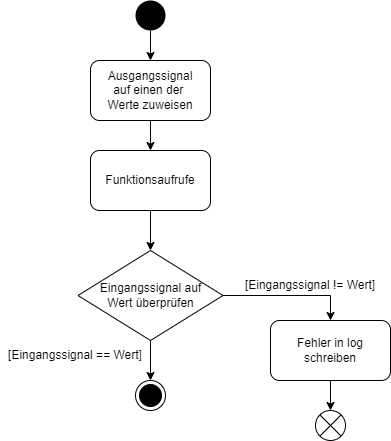
\includegraphics[scale=.6,]{Bilder/Quicktest/QuicktestLogik.drawio.png}
\caption{Quicktest Logik \cite[vgl.][]{quicktestc}}
\end{figure}











% Schnittstellentest:\\ 
	% - Signalverbindungen zwischen der FUs testen:\\
	  % Ausgangssignal einer FU wird zum Eingangssignal der zweiten FU. Test, ob diese Verbindung besteht\\
	% - Testablauf: Ausgangssignal wird auf einen Wert gesetzt und es wird überprüft, ob es als Eingangssignal in der zweiten FU ankommt

% Ein c sharp Skript erzeugt die Datei Quicktest.c\\
% C sharp Skript:\\
% Parsen der xml\_info.xml, darin findet er Out und In Labelverbindungen, sowie Datentyp
% Und Ordner zu .txt Dateien: Funkltionsaufrufe, wo die Verbindung zwischen Ausgangslabel und Eingangslabel hergestellt wird\\

% Quicktest.c wird inklusive des Gesamtprojekts kompiliert und gelinkt\\

% Quicktest.c:\\
% 1. Ausgangslabel einer FU wird auf Werte gesetzt, \\
% 2. Funktionsaufruf, wo die Verbindung der FUs hergestellt wurde\\
% 3. Wert wird am Eingangslabel überprüft\\

% Auf welche Werte gesetzt?\\
% Abhängig vom Datentyp, auf unteren und oberen Grenzwert, 0, physical Min und physical Max 
% Falls float: Fehlertoleranz auf 0.00001f, Überprüfen Eingangslabel auf <  und   > der Fehlertoleranz

% EIN BEISPIEL MIT SDC OUT STB IN IDCFILD ZEIGEN

% Entweder einen Wert oder alle Werte der Schnittstelle

% % Beispiel:
% % m_ACS_Public_ACS_TASKCLASS11.ACS_Out.Umod = (CONV_ONE_FLOAT32)(-3.402E+38);

% % m_PTS_Private_PTS_TASKCLASS11.PTS_In.UmodPhy < (CONV_ONE_FLOAT32)((-3.402E+38) - (0.00001f)) ||
      % % m_PTS_Private_PTS_TASKCLASS11.PTS_In.UmodPhy > (CONV_ONE_FLOAT32)((-3.402E+38) + (0.00001f)) )


% %zweiter Sinn des Quicktests:
% %Überprüfen auf Gleichheit der Datentypen von Ein und Ausgangslabel
% % Überpüfen, ob Signale einer Schnittstelle den gleichen Datentyp haben, typecast der Signale zur Überprüfung

% % Grenzwerte des Datentyps überprüfen, auch mit typecast auf Datentyp
% % 0 Wert überprüfen, ohne typecast

% 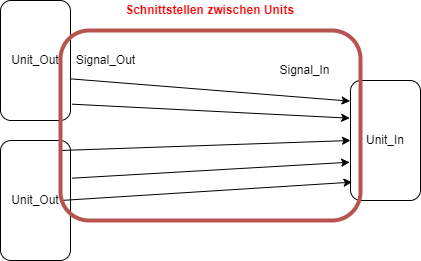
\includegraphics[scale=.6,]{Bilder/Quicktest/AnalyseQuicktest.drawio.png}
% \textbf{Bildinfo Schnittstellen:\\
% Klärung, was eine Schnittstelle ist}